\subsection{Plane strain confined compression -- Excavation in homogeneous media}
\label{subsec:Me2}

\subsubsection{Definition}
\label{subsubsec:Me2_def}

This is the second step of the simulation described in the previous section, Sec.~\ref{subsec:Me1}. A long cylindrical tunnel is driven in the rock mass, which is schematically shown in Fig.~\ref{Me_fme:excav}.
\begin{figure}[!thb]
  \begin{center}
  \epsfig{figure=PART_II/M/ex_plate.eps,width=5.5cm, height=5.5cm}
  \end{center}
  \caption{Excavation in rock mass }
  \label{Me_fme:excav}
\end{figure}


\subsubsection{Solution}
\label{subsubsec:Me2_sol}

The deformation due to the excavation is simulated under the assumption of plane strain. Finite element mesh, initial conditions and material parameters are the same as specified in Sec.~\ref{subsec:Me1}. The tunnel has a radius of $5\,\mbox{m}$. The released loading approach is applied to simulate the excavation.

\subsubsection{Results}
\label{subsubsec:Me2_res}

Fig.~\ref{Me_fig:e2cont} shows the distribution of vertical displacements and coefficients of the stress tensor in the domain after excavation.
\begin{figure}[!htb]
  \centering
   \subfigure[Vertical displacement (m)]{
   \includegraphics[width=0.475\textwidth]{PART_II/M/ee_uy.eps}}
   \subfigure[Horizontal stress (MPa)]{
   \includegraphics[width=0.475\textwidth]{PART_II/M/ee_sxx.eps}}
  \caption{Vertical displacements and horizontal stress after excavation}
  \label{Me_fig_modelhm}
\end{figure}
%
\begin{figure}[!htb]
  \centering
   \subfigure[Shear stress (MPa)]{
   \includegraphics[width=0.475\textwidth]{PART_II/M/ee_sxy.eps}}
   \subfigure[Vertical stress (MPa)]{
   \includegraphics[width=0.475\textwidth]{PART_II/M/ee_syy.eps}}
  \caption{Shear stress and vertical stress after excavation}
  \label{Me_fig:e2cont}
\end{figure}
